\documentclass[tikz]{standalone}
\begin{document}

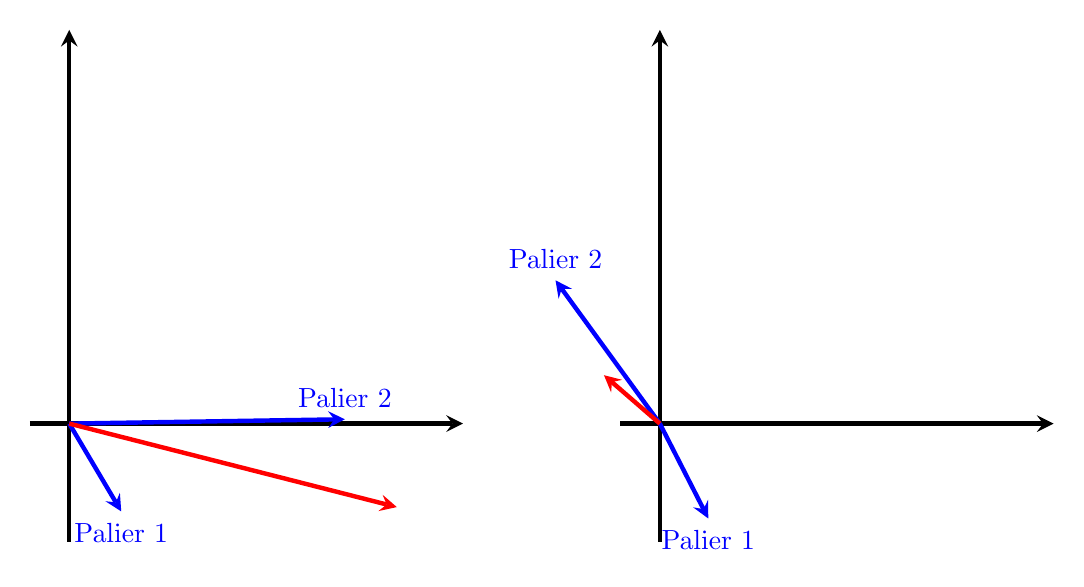
\begin{tikzpicture}[>=stealth]

	\begin{scope}[scale=0.05, ultra thick]
		\draw[->] (-10,0) -- (100,0);
		\draw[->] (0,-30) -- (0,100);
		\draw[->, blue, fill=blue, font=\fontsize{10}{10}\selectfont] (0,0) -- (13.2, -22.3) node[below] {Palier 1};
		\draw[->, blue, fill=blue, font=\fontsize{10}{10}\selectfont] (0,0) -- (70, 1.1) node[above] {Palier 2};
		\draw[->, red, fill=red] (0,0) -- (83.2, -21.2);
	\end{scope}

	\begin{scope}[scale=0.05, shift={(150,0)}, ultra thick]
		\draw[->] (-10,0) -- (100,0);
		\draw[->] (0,-30) -- (0,100);
		\draw[->, blue, fill=blue, font=\fontsize{10}{10}\selectfont] (0,0) -- (12.3, -24.1) node[below] {Palier 1};
		\draw[->, blue, fill=blue, font=\fontsize{10}{10}\selectfont] (0,0) -- (-26.5, 36.4) node[above] {Palier 2};
		\draw[->, red, fill=red] (0,0) -- (-14.2, 12.3);
	\end{scope}

\end{tikzpicture}

\end{document}
